\documentclass[a4paper,11pt]{article}
\usepackage[table]{xcolor}




\usepackage[T1]{fontenc}
\usepackage[normalem]{ulem}
\usepackage{mathtools}
\usepackage{blkarray,bigstrut} 
\usepackage{graphicx,wrapfig,lipsum}
\usepackage{tcolorbox}
\usepackage{enumitem}
\usepackage{array}
\usepackage{algorithm}
\usepackage{algorithmic}
\usepackage{mathpartir}
\usepackage{multirow}
\usepackage{hyperref}
\usepackage{amssymb}
\usepackage{subcaption}
\usepackage{stmaryrd}
\usepackage{color} 


\usepackage{tikz}
\usetikzlibrary{snakes}
\usetikzlibrary{svg.path} 
\usetikzlibrary{calc} 
\usetikzlibrary{shapes}
\usetikzlibrary{shapes.geometric}
\usetikzlibrary{arrows.meta}
\usetikzlibrary{arrows}
\usetikzlibrary{decorations.text,decorations.markings}
% % % % 

%%%%%%%%%%Packages for adaoption%%%

% \usepackage{amsthm} 

%Packages

\input{ldefs}
\newcommand{\highlight}[1]{\textcolor[rgb]{.0,0.0,1.0}{ #1}}

\usetikzlibrary{shapes,arrows}
\newcommand{\THESYSTEM}{\textsf{PsRB}}

% Define block styles
\tikzstyle{decision} = [diamond, draw, fill=blue!20, 
    text width=4.5em, text badly centered, node distance=3cm, inner sep=0pt]
\tikzstyle{block} = [rectangle, draw, fill=blue!20, 
    text width=5em, text centered, rounded corners, minimum height=4em]
\tikzstyle{line} = [draw, -latex']
\tikzstyle{cloud} = [draw, ellipse,fill=red!20, node distance=3cm,
    minimum height=2em]

\begin{document}
\title{Path-sensitive Reachability Bound}

\author{}

\date{}

\maketitle
%
% \input{example_cousot}
% \clearpage
% %
% % 
\section{Path-sensitive Reachability Bound Algorithm}
\label{sec:static_rb}
\subsection{Abstract Transition Graph}
\label{sec:abs_prog}
% \textbf{Step 1: Program Abstract Execution Control Flow Graph}
An \emph{Abstract Transition Graph}, $\absG(c) =(\absV(c), \absE(c))$ for a program $c$ is composed of
a vertex set $\absV(c)$ and an edge set $\absE(c)$.
% For a program $c$, this analysis first generates its abstract execution control flow graph notated as follows,
% \[\absG(c) =(\absV(c), \absE(c))\]
%
\\
Every 
vertex $l \in \absV(c)$ corresponds to a program point, which is a unique
label $l$ of a command in this program.
% $\absV(c)$ is the set of $c$'s all program points,
\\
Each edge $(l, dc, l') \in \absE(c)$ is an abstract transition
between two program points $l, l'$. There is an edge from $l$ to $l'$ if and only if
the command with label $l'$ can execute after the execution of the command with label $l$.
% if and only if there is a control flow between two program points.
Each edge is annotated by a constraint $dc$ generated from the command with label $l$.
% from the set $\dcdom^{\top}$.
% The constraint set contains the different constraints and the boolean expressions. 
% A different constraint is an inequality of form $x \leq y + v$ where 
% $x, y$ are program variables and $v$ is either a 
% % $y \in \mathcal{VAR}$ and $v \in \constdom$.
% % The \emph{Symbolic Variables} $\constdom = \mathbb{N} \cup \inpvar$ is the 
% % set of 
% natural number, the infinity or an input variable. 
\subsection{Program Refinement}
\label{sec:refine}
Three sub-steps:
\begin{enumerate}
\item \textbf{Simple Transition Path}  This step computes the set of all \emph{simple transition paths} for a program $c$.
% \\
% $\tpath \in \paths(\absG(c))$.
% \\
% For a constraint program $\absG(c)$,
% A simple transition path, $\tpath \in \paths(\absG(c))$ for a program c is a path in the abstract transition graph of $c$ that it is either:
% \begin{itemize}
%   \item a simple cyclic path, which starts and ends at the same loop header at location $l$, 
%   and visits only locations inside the natural loop of $l$;
%   %  only one loop (without any nested loop) starting from a loop header at location $l$ and go back to the same $l$;
%   \item or an acyclic path, which starts from a loop header $l$ 
%   % (or the program entrance $l_0$)
% and ends with a different loop header $l'$;
% %  (or the program's exists $\lex$).
% \item or an acyclic path, which starts from a loop header $l$ 
% % (or the program entrance $l_0$)
% and ends the program exists $\lex$;
% %  (or the program's exists $\lex$).
% \item or an acyclic path, which starts from the program entrance $l_0$
% % (or the program entrance $l_0$)
% and ends with a loop header $l$;
% %  (or the program's exists $\lex$).
% \item or an acyclic path, which starts from the program entrance $l_0$
% % (or the program entrance $l_0$)
% and ends the program exists $\lex$;
% %  (or the program's exists $\lex$).
% \end{itemize}
\begin{defn}[Simple Tansition Path]
  A simple transition path
  $\tpath \in \paths(\absG(c))$, is a path on this program's abstract transition graph $\absG(c)$ with 
  \begin{itemize}
  \item a vertices sequence $(l_0, \cdots, l_n)$, where $l_i \in \lvar(c)$ for every $i = 0, \cdots, n$ and
  %
  \item an edge sequence $(e_1, \cdots, e_n)$, where $e_i = (l_{i - 1}, dc_i, l_{i}) \in \absE(c)$ for every $i = 1, \cdots, n$,
  \end{itemize}
  %
  satisfying:
  \begin{itemize}
    \item $l_i \neq l_j$ for every $l_i = l_0, \cdots, l_n$ and $l_j = l_0, \cdots, l_{n - 1}$,
    \item $l_0$ is either the program point of a loop header or the program entrance ($l_0 = 0$),
    \item and $l_n$ is either the program point of a loop header or the program exit ($l_n = \lex$).
  \end{itemize}
  \end{defn}
%
\item \textbf{Repeat Pattern} This step computes the set of all the \emph{repeat patterns} for every while loop in a program $c$.
% \\
% A \emph{Repeat Pattern} ($\rprog \in \mathcal{P}({\absG(c)})$) is either a simple path or sequence of repeat patterns of this program $c$. 
% \[
%   \rpattern := \tpath ~|~ \rprepeat(\rpattern) ~|~ \rpattern; \rpattern
% \]
% Every $\rprog'$ with the annotation $\rprepeat$, (for example, $\rpattern = \rprepeat(\rpattern')$)
% can consecutively execute at least twice.
% Every two sub-repeat patterns following each other in a $\rprog$ can execute in sequence, for example in $\rpattern = \rpattern_1; \rpattern_2$,
% $\rpattern_2$ can execute after $\rpattern_1$.
% Every sub-repeat patterns in the sequence are distinct.
% A \emph{Repeat Pattern},
%   $\rpattern \in \mathcal{P}(\paths({\absG(c)}))$ for a program $c$
% % is either a simple path or sequence of repeat patterns of this program $c$. 
%   % is a sequence of simple transition paths with annotations $\rprepeat$
%   % it is a simple path or
%   is either a simple transition paths $\tpath$,
%   or a sub \emph{repeat pattern} $\rpattern'$ with annotation $\rprepeat$,
%   or a sequence of sub \emph{repeat pattern}s $\rpattern_1; \cdots; \rpattern_n$ satisfying,
%   % \[
% %   \rpattern := \tpath ~|~ \rprepeat(\rpattern) ~|~ \rpattern; \rpattern
% % \]
% \begin{itemize}
% \item If $\rpattern$ has the annotation $\rprepeat$, i.e., $\rprepeat(\rpattern)$,
% then can consecutively execute at least twice w.r.t. some initial trace.
% \item
% If $\rpattern$ is a sequence of sub-repeat patterns,
% i.e.,  $\rpattern = \rpattern_0; \cdots; \rpattern_n$,
% then every two sub-repeat patterns following each other in this sequence
% % i.e., $\rpattern_1; \rpattern_2$, 
% can execute after each other,
% % can execute in sequence, for example in ,
% i.e., 
% $\rpattern_i$ can execute after $\rpattern_{i - 1}$ for every $i = 1, \cdots, n$.
% % $\rpattern_2$ can execute after $\rpattern_1$.
% \item Every sub-repeat pattern in a sequence is distinct.
% \end{itemize}
% \begin{defn}[Repeat Pattern of A Program]
%   \label{def:repeat-pattern}
%   % Given a abstract transition graph $\absG(c)$,
%   % $\rpattern$ is a \emph{Repeat Pattern} of $\absG(c)$ if and only if, 
%   A \emph{Repeat Pattern},
%   $\rpattern \in \mathcal{P}(\paths({\absG(c)}))$ for a program $c$
% % is either a simple path or sequence of repeat patterns of this program $c$. 
%   is 
%   % \todo{
%   % % it is a simple path or
%   % is either a simple transition paths $\tpath$,
%   % or a sub \emph{repeat pattern} $\rpattern'$ with annotation $\rprepeat$,
%   % or a sequence of sub \emph{repeat pattern}s $\rpattern_0; \cdots; \rpattern_n$ ==> }
%   \highlight{a sequence of simple transition paths $\tpath$ with annotation $\rprepeat$ on certain sub-sequence}
%   % a sequence of \emph{repeat pattern}
%   % has the following forms,
%   % \[
%   %   \tpath ~|~ \rprepeat(\rpattern) ~|~ \rpattern; \rpattern
%   % \] 
%   % and 
%   satisfying,
%   \begin{itemize}
%   \item every sub-sequence is distinct, 
%   i.e., if $\rpattern = \rpattern_1; \cdots; \rpattern_n$, then
%   % $\rpattern_i, \rpattern_j \in \rpattern_1; \cdots; \rpattern_n$, 
%   $\rpattern_i \neq \rpattern_j$ for every $i, j = 1, \cdots, n$;
%   \item 
%   % \todo{every sub pattern with the annotation $\rprepeat$
%   % can consecutively execute at least twice in $c$
%   % %  when executing this program $c$ 
%   % w.r.t. some initial trace, i.e., 
%   % if $\rpattern = \rprepeat(\rpattern')$, 
%   % then $\rpattern'$ can consecutively execute at least twice in $c$
%   % under some initial traces, ==> }
%   % \\
%   \highlight{every sub-sequence $\rpattern'$ that has the annotation $\rprepeat$,
%   i.e., $\rprepeat(\rpattern')$
%   % if and only if
%   {must consecutively execute without being interleaved until its invariant is false};}
%   \item 
%   \highlight{
%     % In a repeat pattern $\rpattern = \rpattern_0; \cdots; \rpattern_n$,
%   every sub-sequence $\rpattern_i$ in $\rpattern$, where  $\rpattern = \rpattern_0; \cdots; \rpattern_n$ can execute
%   after the previous $\rpattern_{i - 1}$'s execution is finished.}
%   \end{itemize}
% \end{defn}
\begin{defn}[Repeat Pattern]
  \label{def:repeat-pattern}
  % Given a abstract transition graph $\absG(c)$,
  % $\rpattern$ is a \emph{Repeat Pattern} of $\absG(c)$ if and only if, 
  A \emph{Repeat Pattern},
  $\rpattern \in \mathcal{P}(\paths({\absG(c)}))$ for a while loop in a program $c$
% is either a simple path or sequence of repeat patterns of this program $c$. 
  is
  % \todo{
  % % it is a simple path or
  % is either a simple transition paths $\tpath$,
  % or a sub \emph{repeat pattern} $\rpattern'$ with annotation $\rprepeat$,
  % or a sequence of sub \emph{repeat pattern}s $\rpattern_0; \cdots; \rpattern_n$ ==> }
  \highlight{a sequence of simple transition paths $\tpath$ with annotations $\rprepeat$ on certain sub-sequences,
  $\rpattern = \rpattern_0; \cdots; \rpattern_n$
  }
  % a sequence of \emph{repeat pattern}
  % has the following forms,
  % \[
  %   \tpath ~|~ \rprepeat(\rpattern) ~|~ \rpattern; \rpattern
  % \] 
  % and 
  satisfying that,
  \begin{itemize}
  \item every sub-sequence is distinct, 
  % i.e., if $\rpattern = \rpattern_0; \cdots; \rpattern_n$, then
  % $\rpattern_i, \rpattern_j \in \rpattern_1; \cdots; \rpattern_n$, 
  $\rpattern_i \neq \rpattern_j$ for every $i, j = 0, \cdots, n$;
  \item 
  % \todo{every sub pattern with the annotation $\rprepeat$
  % can consecutively execute at least twice in $c$
  % %  when executing this program $c$ 
  % w.r.t. some initial trace, i.e., 
  % if $\rpattern = \rprepeat(\rpattern')$, 
  % then $\rpattern'$ can consecutively execute at least twice in $c$
  % under some initial traces,}
  % \\
  \highlight{every sub-sequence $\rpattern'$ that has the annotation $\rprepeat$,
  i.e., $\rprepeat(\rpattern')$
  % if and only if
  always executes consecutively without being interleaved until its invariant is false under all possible initial traces;}
  \item 
  % and every two sub patterns following each other in this sequence can execute after each other w.r.t some initial trace,
  % i.e., if $\rpattern = \rpattern_0; \cdots; \rpattern_n$, then for every $i = 1, \cdots, n$,
  % $\rpattern_i$ can execute after $\rpattern_{i - 1}$ under some initial trace.
  % \\
  \highlight{
    % In a repeat pattern $\rpattern = \rpattern_0; \cdots; \rpattern_n$,
  every sub-sequence $\rpattern_i \in \rpattern$ can execute
  after the previous $\rpattern_{i - 1}$'s execution (or iteration) is finished.}
  \end{itemize}
\end{defn}
% \begin{defn}[Repeat Pattern of A Program]
%   \label{def:repeat-pattern}
%   % Given a abstract transition graph $\absG(c)$,
%   % $\rpattern$ is a \emph{Repeat Pattern} of $\absG(c)$ if and only if, 
%   A \emph{Repeat Pattern},
%   $\rpattern \in \mathcal{P}(\paths({\absG(c)}))$ for a program $c$
% % is either a simple path or sequence of repeat patterns of this program $c$. 
%   is 
%   % \todo{
%   % % it is a simple path or
%   % is either a simple transition paths $\tpath$,
%   % or a sub \emph{repeat pattern} $\rpattern'$ with annotation $\rprepeat$,
%   % or a sequence of sub \emph{repeat pattern}s $\rpattern_0; \cdots; \rpattern_n$ ==> }
%   \highlight{a sequence of simple transition paths $\tpath$ with annotation $\rprepeat$ on certain sub-sequence}
%   % a sequence of \emph{repeat pattern}
%   % has the following forms,
%   % \[
%   %   \tpath ~|~ \rprepeat(\rpattern) ~|~ \rpattern; \rpattern
%   % \] 
%   % and 
%   satisfying,
%   \begin{itemize}
%   \item every sub-sequence is distinct, 
%   i.e., if $\rpattern = \rpattern_1; \cdots; \rpattern_n$, then
%   % $\rpattern_i, \rpattern_j \in \rpattern_1; \cdots; \rpattern_n$, 
%   $\rpattern_i \neq \rpattern_j$ for every $i, j = 1, \cdots, n$;
%   \item 
%   % \todo{every sub pattern with the annotation $\rprepeat$
%   % can consecutively execute at least twice in $c$
%   % %  when executing this program $c$ 
%   % w.r.t. some initial trace, i.e., 
%   % if $\rpattern = \rprepeat(\rpattern')$, 
%   % then $\rpattern'$ can consecutively execute at least twice in $c$
%   % under some initial traces, ==> }
%   % \\
%   \highlight{every sub-sequence $\rpattern'$ that has the annotation $\rprepeat$,
%   i.e., $\rprepeat(\rpattern')$
%   % if and only if
%   {must consecutively execute without being interleaved until its invariant is false};}
%   \item 
%   \highlight{
%     % In a repeat pattern $\rpattern = \rpattern_0; \cdots; \rpattern_n$,
%   every sub-sequence $\rpattern_i$ in $\rpattern$, where  $\rpattern = \rpattern_0; \cdots; \rpattern_n$ can execute
%   after the previous $\rpattern_{i - 1}$'s execution is finished.}
%   \end{itemize}
% \end{defn}
% \begin{defn}[Repeat Pattern of A Program]
%   \label{def:repeat-pattern}
%   Given a constraint program $\absG(c)$,
%   $\rpattern(c)$ is a \emph{Repeat Pattern} of $\absG(c)$ if and only if, it is a simple path or
%   a sequence of \emph{repeat pattern}
%   has the following syntax
%   \[
%     \rpattern := \tpath ~|~ \rprepeat(\rpattern) ~|~ \rpattern; \rpattern
%   \] 
%   and satisfying,
%   \begin{itemize}
%   \item every sub-repeat pattern $\rpattern' \in \rpattern(c)$ with the annotation $\rpattern$
%   can consecutively execute twice
%   %  when executing this program $c$ 
%   w.r.t. some initial trace,
%   \item every sub-repeat patter in a sequence is distinct, i.e., $\rpattern(c) = \rpattern_1; \cdots; \rpattern_n$ and 
%   % $\rpattern_i, \rpattern_j \in \rpattern_1; \cdots; \rpattern_n$, 
%   $\rpattern_i \neq \rpattern_j$ for every $i, j = 1, \cdots, n$,
%   \item and every two continuous sub-repeat patters in a sequence can execute after each other w.r.t some initial trace,
%   i.e., $\rpattern(c) = \rpattern_1; \cdots; \rpattern_n$ and for every $i = 1, \cdots, n$,
%   $\rpattern_i$ can execute after $\rpattern_{i - 1}$ under some initial trace.
%   \end{itemize}
% \end{defn}
%
\item \textbf{Refined Program\footnote{For concise, the annotation $\rpchoose{}$ is omitted if there is only one repeat pattern in this set.}}.
% \\
% This step computes the refined program for a program $c$ by composing the
% repeat pattern set of every while loop and the simple transition paths not in any loop.
This step computes the refined program for a program $c$ by composing the
repeat pattern set of every while loop and the simple transition paths not in any loop.
\\
% A \emph{Refined Program} for a program $c$, ($\rprog \in \mathcal{P}(\mathcal{P}(\absG(c)))$),
% is either a repeat pattern , or a set of refined programs, or sequence of refined program
% % ($\rprog \in \mathcal{P}({\absG(c)})$) is either a simple path or sequence of repeat patterns. 
% \[
%   \rprog :=  \rpattern ~|~ \rpchoose{\rprog} ~|~ \rprog; \rprog.
% \]
A \emph{Refined Program} for a program $c$, $\rprog$
%  ($\rprog \in \mathcal{P}(\mathcal{P}(\paths(\absG(c))))$),
% \todo{is either a repeat pattern $\rpattern$,
% or a set of refined programs with annotation $\rpchoose{ \cdots }$, or sequence of refined program $\rprog; \rprog$
% ==>}
has the form $\rprog = \rprog_0; \cdots; \rprog_n$ where each sub-refined program $\rprog_i \in \rprog$
is either a simple transition path, or a set of repeat patterns with annotation $\kw{choose}$.
It is guaranteed to have certain properties by the computation algorithm in the full version.
% % A \emph{Refined Program} for a program $c$, ($\rprog \in \mathcal{P}(\mathcal{P}(\absG(c)))$),
% % is either a repeat pattern, or a set of refined programs, or sequence of refined program
% % % ($\rprog \in \mathcal{P}({\absG(c)})$) is either a simple path or sequence of repeat patterns. 
% % \[
% %   \rprog :=  \rpattern ~|~ \rpchoose{\rprog} ~|~ \rprog; \rprog.
% % \]
% % It satisfies,
% % \begin{itemize}
% %   \item every sub-refined program in a same set with annotation $\rpchoose{\cdots}$ starts and ends with the same control location,
% %   \item and for every two sub-refined programs following each other in a sequence,
% %     the first refined program's ending control location is the same 
% %     as the starting control location of the second refined program.
% %     For example if
% %     $\rprog = \rprog_0; \cdots; \rprog_n$,
% %     $\rpattern_1 \in \rprog_i$
% %     and $\rpattern_2 \in \rprog_{i + 1}$,
% %     then $\rpattern_1$ ends with the same control location as $\rpattern_2$'s starting location.
% % \end{itemize}
% A \emph{Refined Program} for a program $c$, ($\rprog \in \mathcal{P}(\mathcal{P}(\paths(\absG(c))))$),
% is either a repeat pattern $\rpattern$,
% or a set of refined programs with annotation $\rpchoose{ \cdots }$, or sequence of refined program $\rprog; \rprog$
% satisfying,
% \begin{itemize}
%   \item every refined 
%   programs in a same set, $\rpchoose{ \cdots }$
%   %  with annotation $\rpchoose{\cdots}$ 
%   starts and ends with the same control location,
%   \item and for every two sub-refined programs following each other in a sequence,
%     the first refined program's ending control location is the same 
%     as the starting control location of the second refined program.
%     i.e., if
%     $\rprog = \rprog_0; \cdots; \rprog_n$,
%     % $\rpattern_1 \in \rprog_i$
%     % and $\rpattern_2 \in \rprog_{i + 1}$,
%     then all the transition paths in $\rprog_i$ ends with the same control location as 
%     the $rprog_{i + 1}$'s transition paths' starting location.
% \end{itemize}
% \begin{defn}[Refined Program of A Program]
%   % Given a abstract transition graph $\absG(c)$,
%   % its \emph{Refined Program} is either a repeat pattern, or a set of refined program, or sequence of refined program has
%   % the following syntax,
%   % \[
%   %   \rprog :=  \rprepeat ~|~ \rpchoose{\rprog} ~|~ \rprog; \rprog.
%   % \]
%   A \emph{Refined Program} for a program $c$, $\rprog \in \mathcal{P}(\mathcal{P}(\paths(\absG(c))))$
%   is 
%   % \todo{either a repeat pattern $\rpattern$,
%   % or a set of sub-refined programs $\{\rprog_1, \cdots, \rprog_m\}$ with annotation $\kw{choose}$,
%   % or a sequence of sub-refined program $\rprog; \rprog$.
%   % It satisfies that for every sub-refined program $\rprog' \in \rprog$ ==>}
%   \highlight{a sequence of sets of repeat patterns with annotation $\kw{choose}$ satisfying}
%   % $\rprog = \rprog_1, \cdots; \rprog_n$ and
%   % $\rprog_i = \{\rpattern_{0}; \cdots; \rpattern_{i_n}\}$, $n, i_n \in \mathbb{N}$ and
%   \begin{itemize}
%     \item $\rprog$ has the form $\rpchoose{\rpattern_1, \cdots }; \rpchoose{\rpattern'_1, \cdots }; \cdots$.
%   \item 
%   % \todo{every
%   %  $\rpattern, \rpattern' \in \rpchoose{\rprog_1, \cdots, \rprog_m}$,
%   %  then all the $\rprog_1, \cdots, \rprog_m$ have the same starting and ending label,==>}
%    \highlight{Every $\rpattern$ in the same set,
%    $\rpattern \in \rpchoose{\rprog_1, \cdots, \rprog_m}$ 
%    starts from the same program point $l$ and ends at the same program point $l'$ for $l, l' \in \lvar(c)$.}
%   \item 
%   % \todo{if $\rprog' = \rprog_1; \rprog_2$, then
%   % % and for every $\rpattern_1 \in \rprog_i$ and $\rpattern_2 \in \rprog_{i + 1}$,
%   % $\rprog_1$'s ending label is the same label as $\rprog_2$'s starting label. ==>}
%   If two repeat patterns from two different sets following each other in the sequence,
%   $\rpattern \in \rpchoose{\rpattern_1, \cdots}$, $\rpattern' \in \rpchoose{\rpattern_1', \cdots}$ and
%   $\rprog = \cdots, \rpchoose{\rpattern_1, \cdots}; \rpchoose{\rpattern_1', \cdots}, \cdots$,
%   then $\rpattern$ ends at the program point $l$ from which $\rpattern'$ starts.
%   \end{itemize}
% \end{defn}
% \\
% \begin{defn}[Refined Program of A Program]
%   Given a constraint program $\absG(c)$,
%   its \emph{Refined Program} is either a repeat pattern, or a set of refined program, or sequence of refined program has
%   the following syntax,
%   \[
%     \rprog :=  \rprepeat ~|~ \rpchoose\left\{\rprog\right\} ~|~ \rprog; \rprog.
%   \]
%   It satisfies that for every sub refined program $\rprog' \in \rprog$
%   % $\rprog = \rprog_1, \cdots; \rprog_n$ and
%   % $\rprog_i = \{\rpattern_{0}; \cdots; \rpattern_{i_n}\}$, $n, i_n \in \mathbb{N}$ and
%   \begin{itemize}
%   \item if
%    $\rprog' = \rpchoose\left\{\rprog_1, \cdots, \rprog_m \right\}$,
%    then all the $\rprog_1, \cdots, \rprog_m$ have the same starting and ending label,
%   \item if $\rprog' = \rprog_1; \rprog_2$, then
%   % and for every $\rpattern_1 \in \rprog_i$ and $\rpattern_2 \in \rprog_{i + 1}$,
%   $\rprog_1$'s ending label is the same label as $\rprog_2$'s starting label.
%   \end{itemize}
% \end{defn}
%
%  annotation for two branches of $\eif$.
% them into
%  of this loop header
%s
% \textbf{Theorem Guarantee.}
% Soundness of the refinement.
\end{enumerate}
\subsection{Ranking Function/ Local Bound Computation}
\label{sec:ranking}
% It estimates the bounds on the maximum value of counter variables, and
% the iteration times
% % of the ranks / local bounds 
% for each edge in the constraint program $\absG(c)$, using the method in \cite{sinn2017complexity}.
% There are three sub-steps as follows.
This step computes a 
\textbf{ranking function / local bound
\footnote{\textbf{ranking function} is the named used in \cite{SinnZV14}
and \textbf{local bound} is the name used in \cite{ZulegerGSV11}, \cite{sinn2017complexity}.
We refer to the two names as the same meaning in this paper.}}
for each edge in the abstract transition graph $\absG(c)$ of a program $c$.
Then it estimates the bound on the maximum value of each ranking function / local bound as well as
% , and
the bound on the execution times of the corresponding edge in a path-insensitive manner.
\\
For each edge $\absevent \in \absG(c)$,
$\locbound(\absevent)$ is the \textbf{Ranking Function} assigned to $\absevent$.
\\
For each ranking function $\locbound(\absevent)$, $\varinvar(\locbound(\absevent))$ is
the \textbf{Ranking Function Bound} on its maximum value.
\\
For each edge $\absevent \in \absG(c)$, the $\absclr(\absevent)$ is the \textbf{Path-insensitive Transition Bound}
% $\absclr(\absevent) \in \mathcal{A}_{\lin}$ 
% for the edge $\absevent \in \absG(c)$,
% is the bound 
on the execution times of this edge in $c$.
% \textbf{Step1: Variable Constraint Collection:}
% Identify the abstract events where each variable is increased, decreased and reset:
% \\
% $\inc: \mathcal{VAR} \to \mathcal{P}(\absE(c)) $
% the set of the abstract events where the variable increase.
% \\
% $\inc(x) = \{(e, c) | e = (l, x' \leq x + c, l') \land e \in \absE(c)\}$
% \\
% $\reset: \mathcal{VAR} \to \mathcal{P}(\absE(c)) $
% The set of the abstract events where the variable is reset.
% \\
% $\dec: \mathcal{VAR} \to \mathcal{P}(\absE(c)) $
% The set of abstract events where the variable decrease.
% \\
% \textbf{{Step2: Assign Ranks / Local Bound to Edges}}
% $\locbound: \absE(c) \to \mathcal{VAR} \cup \constdom$.
%  \\
% \textbf{Step3: Ranks / Local Bounds Estimation}
% Estimating the bounds on the (ranks'/ local bounds') maximum value.
% % , the 
% \\ 
% $ \varinvar: \mathcal{VAR} \cup \constdom \to \mathcal{A}_{\lin}$
% % \\
% % $\absclr: \absE(c) \to \mathcal{A}_{\lin}$
% \\
% $Incr(x) \triangleq \sum\limits_{(e, c) \in \inc(x)}\{\absclr(\absevent) \times v\}$
% \\
% It estimates the bounds on the maximum value of counter variables, and
% the iteration times
% % of the ranks / local bounds 
% for each edge in the constraint program $\absG(c)$, using the method in \cite{sinn2017complexity}.
% % \\
% % computing the loop bound in a path-insensitive way as the base step.
% % \\ 
% % $ \varinvar: \mathcal{VAR} \cup \constdom \to \mathcal{A}_{\lin}$
% \\
% $\absclr: \absevent \to \mathcal{A}_{\lin}$
% \\
% \textbf{Theorem Guarantee.}
% Soundness of the Path-Insensitive Local Bound / Rank Estimation.
%  Require Variable Bound Computation.
\subsection{Outside-In Algorithm}
\label{sec:outinalg}
% For the refined program $\rprog \in \mathcal{RP}$, the \textbf{Outside-In Algorithm} ($\outinB: \rprog \to \mathcal{A}_{in}$)
% computes the \emph{OutIn} bound on the iteration numbers of every repeat pattern in this program.
% \\
% It is called \emph{OutIn} bound because for a repeat pattern $\rpattern$ nested
% in another repeat pattern $\rpattern' = \rprepeat(\rpattern)$,
% this value only bounds the iteration number of $\rpattern$ inside $\rpattern'$ by assuming $\rpattern'$ executes once.
For every repeat pattern $\rpattern$ in a refined program $\rprog$, 
this algorithm
computes the \textbf{Outside-In} bound, $\outinB(\rprog, \rpattern) \in \mathcal{A}_{in}$ on its iteration numbers locally.
%  of every repeat pattern 
\\
$\outinB(\rprog, \rpattern)$ is the \textbf{Outside-In} bound for a repeat pattern $\rpattern$ in the sense that
% for a repeat pattern 
if $\rpattern$ is nested
in another repeat pattern, i.e., $\rpattern' = \rprepeat(\rpattern)$,
it only bounds $\rpattern$'s iteration number within $\rpattern'$ by assuming that $\rpattern'$ executes once.
% \highlight{\textbf{Notations / Operators:}}
\\ \highlight{Computation:}
\\
The \textbf{Outside-In} bound, $\outinB(\rprog, \rpattern) \in \mathcal{A}_{in}$
for a repeat pattern $\rpattern$ in a refined program $\rprog$
is computed recursively as follows,
% for every nested repeat patterns in $\rprog$,
% \\
% $\outinB(\rpchoose{\rprog_1, \cdots, \rprog_m}) =  \max\{\outinB(\rprog_1), \cdots, \outinB(\rprog_m)\}$
\\
$\outinB(\rprog, \rprepeat({\rpattern})) =  \frac{\rfinit(\rprog, \rpattern) - \rffinal(\rprog, \rpattern)}{\varGD(\rprog, \rpattern)}$
\\
$\outinB(\rprog, \rpattern_1; \rpattern_2) =  \outinB(\rprog, \rpattern_1)+ \outinB(\rprog,  \rpattern_2)$
\\
$\outinB(\rprog, \tpath) =  1$.
\\
% The \emph{State}: 
% $\absstate \in \mathcal{P}(\dcdom^{\top})$ : conjunctions of the edge annotations.
% %  constraints.
% \\
% For a refined program ($\rprog$), there are the 
% \\
% \emph{Initial State} ($\rfinit(\rprog)$), 
% \emph{Final State} ($\rffinal(\rprog)$), and \emph{Next State} ($\rfnext(\rprog)$)  $\in \absstate$.
% % The \emph{Initial State}: $\rfinit : \rprog \to \absstate $.
% \\
% The \emph{Variable Grade Decedent}: $\varGD : \rprog \to \mathcal{A}_{in}$, is the set of the variables' variation in one iteration;
% % The \emph{Initial State}: $\rfinit : \rprog \to \absstate $.
The computations for $\rfinit(\rprog, \rpattern)$,
$\rffinal(\rprog, \rpattern)$, $\rfnext(\rprog, \rpattern)$ and $\varGD(\rprog, \rpattern) \in \mathcal{A}_{in}$
are in the full version.
\subsection{Inside-Out Algorithm}
\label{sec:inoutalg}
% For the refined program $\rprog \in \mathcal{RP}$, the \textbf{Inside-Out Algorithm}
% computes the reachability-bound on the execution numbers for every simple transition path $\tpath$ in this program $\rprog$,
% through the following steps.
For every simple transition path $\tpath$ in a refined program $\rprog$, 
this algorithm
computes the \textbf{Inside-Out} bound, $\outinB(\rprog, \tpath) \in \mathcal{A}_{in}$
%  on its iteration numbers locally.
% computes the bound
on the execution numbers of $\tpath$ path-sensitively
% for every simple transition path $\tpath$ in this program $\rprog$,
through the following steps.
%
\begin{enumerate}
  \item \emph{Repeat Chain Bound:} $\rpchB(l, \tpath, \rprog) \in \mathcal{A}_{in}$.
  \\
  For every transition path $\tpath$ in a refined program $\rprog$,
  its \emph{Repeat Chain Bound} is the
  bound on its execution numbers inside its closet while loop.
  \item \emph{Relative Loop Bound:} $\lpchB(l, \tpath, \rprog) \in \mathcal{A}_{\lin}$.
  \\
  For every simple transition path $\tpath$
and a loop header at location $l$ in a refined program $\rprog$,
the \emph{Relative Loop Bound} $\lpchB(l, \tpath, \rprog) \in \mathcal{A}_{\lin}$ is a symbolic expression in $\mathcal{A}_{\lin}$.
\\
This expression is a sound bound on the iteration numbers of loop $l$ relative to the simple transition path $\tpath$.
This $\tpath$'s closest enclosing loop has the loop header at $l'$ and $l'$ is nested inside the loop $l$.
% \\
It estimates the iteration numbers of loop $l$ such that during these iterations, the nested loop $l'$ is executed.
%
\item The \emph{Inside-Out Bound} ($\inoutB(\tpath, \rprog) \in \mathcal{A}_{in}$).
\\
For every simple transition path $\tpath \in \rprog$,
its \emph{Inside-Out Loop Bound}
 $\inoutB(\tpath, \rprog) \in \mathcal{A}_{in}$ is 
% Compute 
the path sensitive reachability-bound on $\tpath$'s execution numbers.

% \highlight{\textbf{Omitted Computations:}}
\begin{defn}[{Inside-Out Loop Bound}]
  \label{def:outin_bound}
  Given a refined program $\rprog$, for every transition path $\tpath \in \rprog$, 
  its \emph{Inside-Out Loop Bound}
  $\inoutB(\tpath, \rprog)$ is 
 % Compute 
$
  \prod\limits_{l \in \lpch(\tpath, \rprog)} \rpchB(l, \tpath, \rprog).
% lpRB(\rprog_i, \tpath) 
% ~ \middle\vert~ l \in lp\mathcal{C}(\tpath) \right
$
\end{defn}
% For $chain \in rpchain(\tpath)$:
% where $lpchains(\tpath)$ is set of $lpchains(\tpath)$ containing all the loop chains of $\tpath$.
\end{enumerate}
\subsection{Path-sensitive Reachability-Bound Computation}

For every program control location $l \in \lvar(c)$, with $\rprog$ as its refined program,
%  in a program $c$,
its path-sensitive reachability-bound ($\psRB(l, \rprog)$) is a symbolic sound bound on the executing times of $l$.
 \begin{defn}
  \label{def:label_psrb}
Given a program $c$ with its refined program $\rprog \in \mathcal{RP}$
%  with 
% \emph{Global Loop Bound} $\inoutB(\tpath)$
% computed for its every transition path $\tpath \in \rprog$  notated by $\inoutB(\tpath)$,
%  for each of its transition path $\tpath \in \rprog$ 
% with the \emph{Global Loop Bound}
% computed as above, notated by $\inoutB(\tpath)$.
the $\psRB(c, l)$ for every label $l \in \lvar(c)$ is computed as follows,
\\
\[ \psRB(c, l) = \sum\limits_{\tpath \in \rprog \land 
l \in \tpath} \inoutB(\tpath)\]
 \end{defn}
% % % % 
% \section{Examples}
% \label{sec:example}
\section{Example I: The Two Paths While Loop Example}
\begin{example}[While with Two Counters]
  \label{ex:twoCountersWhile}
  %
  { \small
  \begin{figure}
  \centering
  \begin{subfigure}{.4\textwidth}
    \begin{centering}
    {\small
    $
    \begin{array}{l}
      \kw{twoCountersWhile}(n, m) \triangleq \\
    \clabel{ \assign{i}{n} }^{0} ; \\
    \clabel{ \assign{j}{0} }^{1} ; \\
        \ewhile ~ \clabel{i > 0}^{2} ~ \edo ~ \\
        \qquad \Big(
          \eif(\clabel{j < m}^{3}, \\
          \qquad \qquad \clabel{\assign{j}{j + 1}}^{4}; 
          \clabel{\assign{i}{i - 1}}^{5},\\
          \qquad \qquad \clabel{\assign{j}{0}}^{6});
          \Big)
        \end{array}
        $
    }
    \caption{}
    \end{centering}
    \end{subfigure}
  \begin{subfigure}{.5\textwidth}
    \begin{centering}
  %   \todo{abstract-cfg for two round}
  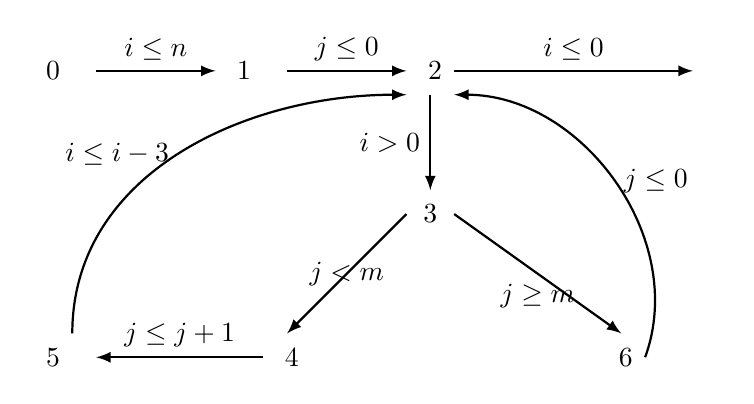
\begin{tikzpicture}[scale=\textwidth/20cm,samples=200]
  \draw[] (-8, 10) circle (0pt) node{{ $0$}};
  \draw[] (-4, 10) circle (0pt) node{{ $1$}};
  \draw[] (0, 10) circle (0pt) node{{ $2$}};
  \draw[] (0, 7) circle (0pt) node{{$3$}};
  \draw[] (-3, 4) circle (0pt) node{{ $4$}};
  \draw[] (-8, 4) circle (0pt) node{{ $5$}};
  \draw[] (4, 4) circle (0pt) node{{ $6$}};
  % Counter Variables
  \draw[] (6, 10) circle (0pt) node {\textbf{$\lex$}};
  % \draw[] (6, 4) circle (0pt) node {{ $ex$}};
  %
  % Control Flow Edges:
  \draw[ thick, -latex] (-7, 10)  -- node [above] {$i \leq n$}(-4.5, 10);
  \draw[ thick, -latex] (-3, 10)  -- node [above] {$j \leq 0$}(-0.5, 10);
  \draw[ thick, -latex] (0, 9.5)  -- node [left] {$i > 0$} (0, 7.5) ;
  \draw[ thick, -latex] (0.5, 7)  -- node [below] {$ j \geq m $}  (4, 4.5);
  \draw[ thick, -latex] (-7.5, 4.5)  to  [out=90,in=180]  node [left] {$i \leq i - 3$ }(-0.5, 9.5);
  \draw[ thick, -latex] (4.5, 4)  to  [out=70,in=0]   node [right] {$j \leq 0 $}(0.5, 9.5);
  \draw[ thick, -latex]  (-0.5, 7) -- node  {$j < m$}  (-3, 4.5) ;
  \draw[ thick, -latex]  (-3.5, 4) -- node [above] {$j \leq j + 1$}  (-7, 4) ;
  \draw[ thick, -latex] (0.5, 10)  -- node [above] {$i \leq 0$}  (5.5, 10);
  % \draw[ thick, -latex] (6, 6.5)  -- node [right] {$\top$} (6, 4.5) ;
  \end{tikzpicture}
  \caption{}
    \end{centering}
    \end{subfigure}
  \caption{
  (a) The Two Paths While Loop Example with Two Coutners
    (b) The Abstract Execution Control Flow Graph}
      \label{fig:twoCountersWhile}
  \end{figure}
  }
\end{example}

\begin{enumerate}
  \item  \textbf{The Abstract Execution Control Flow Graph} is generated in Figure~\ref{fig:twoCountersWhile}(b).

  \item \textbf{Program Rephrase and Refinement}. 
  \\
  The loop free transition paths are computed as follows,
  \[
    \begin{array}{ll}
\tpath_0 = (0 \to 1), (1 \to 2)
&
\tpath_2 = (2 \to 3), (3 \to 6), (6 \to 2)
\\
\tpath_1 = (2 \to 3), (3 \to 4), (4 \to 5), (5 \to 2)
&
\tpath_3 = (2 \to \lex)
\end{array}
\]
\textbf{Rephrased Program}:
\[
\tpath_0 ; LOOP1: \rprepeat(\rpchoose\{\tpath_1, \tpath_2 \}); \tpath_3
\]
\textbf{Refined Program}:
\[
  \tpath_0 ; LOOP1: \rpchoose\{\rprepeat_2(\rprepeat_1(\tpath_1); \tpath_2) , \rprepeat_1(\tpath_1) \}; \tpath_3
  \]
  \item \textbf{Outside-In Algorithm} : Compute Local Bound for Every program and sub programs.
  \[
    \begin{array}{l}
        LB(\tpath_0) = 1
        \\
        LB(\rprepeat_1(\tpath_1)) = m 
        \\
        LB(\rprepeat_2(\rprepeat_1(\tpath_1); \tpath_2)) = \lfloor\frac{n}{m}\rfloor
        \\
        LB(LOOP1: \rpchoose(\rprepeat_2(\cdots), \rprepeat_1(\tpath_1))) 
        = \max\{m, (m  + 1)\times \lfloor\frac{n}{m}\rfloor\}
\end{array}
\]
\item \textbf{Inside-Out Algorithm}
\begin{itemize}
  \item \textbf{Repeat Chain Set}
  \\
  $rp\mathcal{C}(LOOP1, \tpath_1) = \{\rprepeat_1(\tpath_1), \rprepeat_2(\rprepeat_1(\tpath_1); \tpath_2) \to \rprepeat_1(\tpath_1)\}$ \\
  $rp\mathcal{C}(LOOP1, \tpath_2) = \{\rprepeat_2(\cdots; \tpath_2) \to \rprepeat_1(\tpath_1)\}$ \\
  $rp\mathcal{C}(\_, \_) = \emptyset$ 
  % \\
  \item \textbf{{Local Repeat Chain Bound} }for Every Transition Path $\tpath$ on its Repeat Chain
  \\
  $rpLB(LOOP1, \tpath_1) = \max\{m, m \times \lfloor\frac{n}{m}\rfloor\}$ \\
  $rpLB(LOOP1, \tpath_2) = \lfloor\frac{n}{m}\rfloor$ 
  %
  \item \textbf{Loop Chain} Set
  \\
  $lp\mathcal{C}(\tpath_0) = \{\tpath_0\}$ \qquad
  $lp\mathcal{C}(\tpath_1) = \{LOOP1\to \tpath_1\}$ \\
  $lp\mathcal{C}(\tpath_3) = \{\tpath_3\}$ \qquad
  $lp\mathcal{C}(\tpath_2) = \{LOOP1\to \tpath_2\}$ 
  \item \textbf{Nested Loop Bound }for Every Transition Path $\tpath$ on its Loop Chain
  \\
  $rpLB(LOOP1, \tpath_1) = \max\{m, m \times \lfloor\frac{n}{m}\rfloor\}$ \quad
  $rpLB(LOOP1, \tpath_2) = \lfloor\frac{n}{m}\rfloor$  \\
  $rpLB(\bot, \tpath_0) = 1$ \quad
  $rpLB(\bot, \tpath_3) = 1$ 
  \item \textbf{Path Sensitive Reachability Bound For Every Transition Path $\tpath$ }
  \\
  $psRB(\tpath_1) = n$ \quad
  $psRB(\tpath_2) = \lfloor\frac{n}{m}\rfloor$ \quad
  $psRB(\tpath_0) = 1$ \quad
  $psRB(\tpath_3) = 1$ 
\end{itemize}
\item Step 7: Path Sensitive Reachability Bound Computation for Every Location
\\
$psRB(\{0, 1\}) = 1$ \qquad
$psRB(\{\lex\}) = 1$ \qquad
$psRB(\{6 \}) = \lfloor\frac{n}{m}\rfloor$ \\
$psRB(\{4, 5 \}) = \max\{m, m \times \lfloor\frac{n}{m}\rfloor\}$ \quad
$psRB(\{3, 2 \}) = \max\{m, m \times \lfloor\frac{n}{m}\rfloor\} + \lfloor\frac{n}{m}\rfloor + 1 $ \\
\end{enumerate}
\section{Example II: Nested Loop with Related Iterator}
\begin{example}[Nested Loop with Related Iterators]
  \label{ex:threeNestedWhile}
  %
  %
  { \small
\begin{figure}
\centering
\begin{subfigure}{.4\textwidth}
  \begin{centering}
  {\footnotesize
  $
  \begin{array}{l}
      \kw{relatedNestedWhile}(n, m, N) \triangleq \\
      \clabel{ \assign{i}{0} }^{0} ; \\
          \ewhile ~ \clabel{i < n}^{1} ~ \edo ~ \\
          \qquad \Big(
           \clabel{\assign{j}{m}}^{2} ;\\
           \qquad \ewhile ~ \clabel{j > 0}^{3} ~ \edo ~ \\
           \qquad \qquad \Big(
            \clabel{\assign{j}{j-1}}^{4};
            \clabel{\assign{w}{i}}^{5};\\
            \qquad \qquad \ewhile ~ \clabel{w < N}^{6} ~ \edo ~
            \Big(
              \clabel{\assign{w}{w + 1}}^{7}
                \Big); \\
                \qquad \qquad \clabel{\assign{i}{w}}^{8}
                \Big); \\
                \qquad \clabel{\assign{i}{i+1}}^{9}
            \Big)
      \end{array}
  $
  }
  \caption{}
  \end{centering}
  \end{subfigure}
\begin{subfigure}{.5\textwidth}
  \begin{centering}
%   \todo{abstract-cfg for two round}
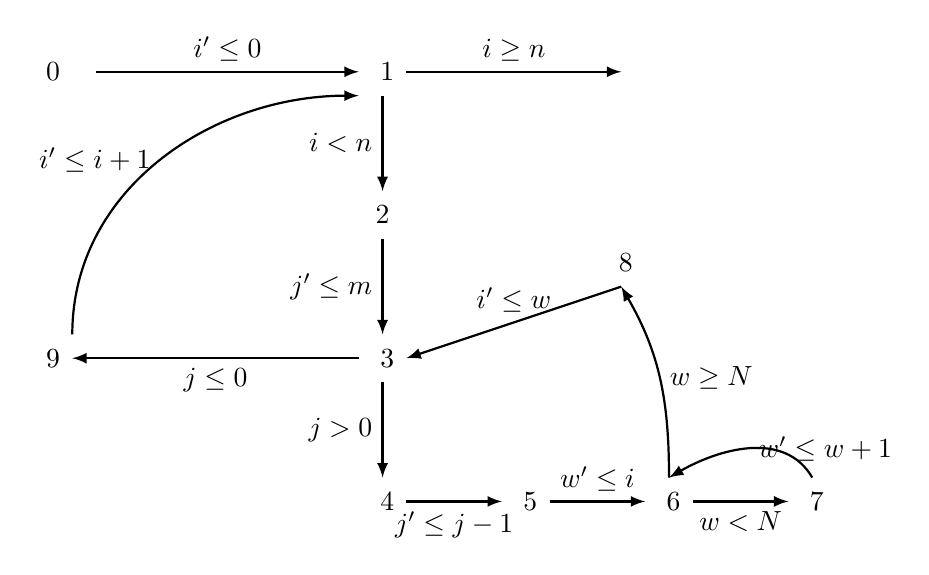
\begin{tikzpicture}[scale=\textwidth/20cm,samples=200]
\draw[] (-7, 10) circle (0pt) node{{ $0$}};
\draw[] (0, 10) circle (0pt) node{{ $1$}};
\draw[] (6, 10) circle (0pt) node {{$\lex$}};
\draw[] (0, 7) circle (0pt) node{{$2$}};
\draw[] (0, 4) circle (0pt) node{{ $3$}};
\draw[] (-7, 4) circle (0pt) node{{ $9$}};
\draw[] (0, 1) circle (0pt) node{{ $4$}};
\draw[] (3, 1) circle (0pt) node{{ $5$}};
\draw[] (6, 1) circle (0pt) node{{ $6$}};
\draw[] (9, 1) circle (0pt) node{{ $7$}};
\draw[] (5, 6) circle (0pt) node{{ $8$}};
% Counter Variables
%
% Control Flow Edges:
\draw[ thick, -latex] (-6, 10)  -- node [above] {$i' \leq 0$}(-0.5, 10);
\draw[ thick, -latex] (0, 9.5)  -- node [left] {$i < n$} (0, 7.5) ;
\draw[ thick, -latex] (0, 6.5)  -- node [left] {$j' \leq m$} (0, 4.5) ;
\draw[ thick, -latex] (0, 3.5)  -- node [left] {$j > 0$} (0, 1.5) ;
\draw[ thick, -latex] (-0.5, 4)  -- node [below] {$j \leq 0$} (-6.5, 4) ;
\draw[ thick, -latex] (-6.5, 4.5)  to  [out=90,in=180]  node [left] {$i' \leq i + 1$ }(-0.5, 9.5);
\draw[ thick, -latex] (0.5, 10)  -- node [above] {$i \geq n$}  (5, 10);
\draw[ thick, -latex] (0.5, 1)  -- node [below] {$j' \leq j - 1$}  (2.5, 1);
\draw[ thick, -latex] (3.5, 1)  -- node [above] {$w' \leq i$}  (5.5, 1);
\draw[ thick, -latex] (6.5, 1)  -- node [below] {$w < N$}  (8.5, 1);
\draw[ thick, -latex] (6, 1.5)  to [out=90,in=-60] node [right] {$w \geq N$}  (5, 5.5);
\draw[ thick, -latex] (9, 1.5)  to  [out=120,in=30] node [right] {$w' \leq w + 1$}  (6, 1.5);
\draw[ thick, -latex] (5, 5.5)  to  node [above] {$i' \leq w$ }(0.5, 4);
\end{tikzpicture}
\caption{}
  \end{centering}
  \end{subfigure}
\caption{
(a) The Example of Nested Loop with Related Iterators
  (b) The Abstract Execution Control Flow Graph}
    \label{fig:threeNestedWhile}
\end{figure}
}
\end{example}

\begin{enumerate}
  \item  \textbf{The Abstract Control Flow Graph}: Figure~\ref{fig:threeNestedWhile}(b).

  \item \textbf{Program Refinement}
  \\
  {Simple Transition Paths:}
  %  are computed as follows,
  \\
$
      \begin{array}{llll}
          \tpath_0 = (0 \to 1)
          &
          \tpath_1 = (1 \to 2 \to 3)
          &           
          \tpath_2 = (3 \to 4 \to 5 \to 6)
          &
          \tpath_3 = (6 \to 7 \to 6)
          \\
          \tpath_6 = (1 \to \lex)
          &
          \tpath_4 = (6 \to 8 \to 3)
          &
          \tpath_5 = (3 \to 9 \to 1)
      \end{array}
$
  \\
  Refined Program:
\\
$
  \rprog = \tpath_0 ; 
1: \rprepeat(\tpath_1; 3: \rprepeat(\tpath_2; 6: \rprepeat(\tpath_3); \tpath_4); \tpath_5); \tpath_6
$
\\
Let $\rprog_1 = \rprepeat(\tpath_1; 3: \rprepeat(\tpath_2; 6: \rprepeat(\tpath_3); \tpath_4); \tpath_5)$
\\
$\rprog_3 = \rprepeat(\tpath_2; 6: \rprepeat(\tpath_3); \tpath_4)$
\\
$\rprog_6 = \rprepeat(\tpath_3)$
  \item {Path Local Reachability-bound}:
\\
$\outinB(1: \rprog_1, \tpath_1) = n - N$ \quad
$\outinB(1: \rprog_1, \tpath_5) = n - N$ \quad
$\outinB(3: \rprog_3, \tpath_2) = m$ \\
$\outinB(3: \rprog_3, \tpath_4) = m$ \quad
$\outinB(6: \rprog_6, \tpath_3) = N$ \quad
%
\\
Loop Bounds:
\\
$BD(\tpath_0) = 1$
\quad
$BD(\tpath_6) = 1$
\quad
$BD( \rprepeat(\tpath_3)) = N $
\quad
$BD(\rprog_3) = m $
\quad
$BD(\rprog_1) = n - N $
%
\item Loop Reachability-bound:
\\
\highlight{
$\lpchB(1: \rprog_1, \tpath_1) = n - N$ \quad
$\lpchB(1: \rprog_1, \tpath_5) = n - N$ \quad
$\lpchB(1: \rprog_1, \tpath_2) = n$ \\ 
$\lpchB(1: \rprog_1, \tpath_4) = n$ \quad
$\lpchB(1: \rprog_1, \tpath_3) = 1$ \quad
$\lpchB(3: \rprog_3, \tpath_4) = m$ \\
$\lpchB(3: \rprog_3, \tpath_2) = m$ \quad
$\lpchB(3: \rprog_3, \tpath_3) = 1$ \quad 
$\lpchB(6: \rprog_6, \tpath_3) = N$
}
%
%
\item Path Global Reachability-bound:
\\
$\inoutB(\rprog, \tpath_1) = n - N$ \quad
$\inoutB(\rprog, \tpath_2) = n \times m$ \quad
$\inoutB(\rprog, \tpath_0) = 1$ 
\quad
$\inoutB(\rprog, \tpath_5) = n - N$ \quad
$\inoutB(\rprog, \tpath_4) = n \times m$ \quad
$\inoutB(\rprog, \tpath_6) = 1$ 
\quad
$\inoutB(\rprog, \tpath_3) = N$
%
\item The Reachability-bound:
\\
$\psRB(0) = \psRB(\lex) = 1$ \quad
$\psRB(1) = n - N + 1$ \quad
$\psRB(2) = \psRB(9) = n - N$ \quad
$\psRB(7) = N$
\\
$\psRB(3) = n - N + n \times m$ \quad
$\psRB(4) = \psRB(5) = \psRB(8) = n \times m$ \quad
$\psRB(6) = N + n \times m$ 
\end{enumerate}
%

% \clearpage
% \appendix
% \addcontentsline{toc}{section}{Appendices}
% \section*{Appendices}


\clearpage
\bibliographystyle{plain}
\bibliography{main.bib}
\end{document}



